% Created 2017-03-06 Mon 14:33
% Intended LaTeX compiler: pdflatex
\documentclass[a4paper,11pt]{article}
\usepackage[utf8]{inputenc}
\usepackage[T1]{fontenc}
\usepackage{graphicx}
\usepackage{grffile}
\usepackage{longtable}
\usepackage{wrapfig}
\usepackage{rotating}
\usepackage[normalem]{ulem}
\usepackage{amsmath}
\usepackage{textcomp}
\usepackage{amssymb}
\usepackage{capt-of}
\usepackage{hyperref}
\usepackage[margin=1in]{geometry}
\usepackage{setspace}
\onehalfspacing
\usepackage{parskip}
\usepackage{amsthm}
\usepackage{amsmath}
\usepackage{mathtools}
\usepackage{hyperref}
\usepackage{graphicx}
\usepackage{tabularx}
\usepackage{booktabs}
\hypersetup{colorlinks,citecolor=black,filecolor=black,linkcolor=black,urlcolor=black}
\newtheorem{definition}{Definition}
\newtheorem{theorem}{Theorem}
\newcommand{\rarrowd}[1]{\xrightarrow{\text{ \textit #1 }}}
\DeclareMathOperator*{\plim}{plim}
\newcommand{\plimn}{\plim_{n \rightarrow \infty}}
\usepackage[margin=1in]{geometry}
\usepackage{setspace}
\onehalfspacing
\usepackage{parskip}
\usepackage{amsthm}
\usepackage{amsmath}
\usepackage{mathtools}
\usepackage{hyperref}
\usepackage{graphicx}
\usepackage{tabularx}
\usepackage{booktabs}
\hypersetup{colorlinks,citecolor=black,filecolor=black,linkcolor=black,urlcolor=black}
\setcounter{secnumdepth}{2}
\author{Zheng Tian Zheng Tian}
\date{}
\title{Lecture 5: An Introduction to R Empirical Exercise 3.1}
\hypersetup{
 pdfauthor={Zheng Tian Zheng Tian},
 pdftitle={Lecture 5: An Introduction to R Empirical Exercise 3.1},
 pdfkeywords={},
 pdfsubject={},
 pdfcreator={Emacs 25.1.1 (Org mode 9.0.3)},
 pdflang={English}}
\begin{document}

\maketitle
\setcounter{tocdepth}{1}
\tableofcontents



\section{Getting Started with R}
\label{sec:orgae11015}

\subsection{What is R?}
\label{sec:org924c20f}

R is a free software environment and programming language for
statistical computing and graphics. The website for the R project is
\url{https://www.r-project.org/}.

\subsubsection*{A brief history of development of R}
\label{sec:org0a74503}

\begin{itemize}
\item It originated from Bell Laboratories in the 1970s, as the S
language, from which the commercial version S-Plus was developed
in 1987.

\item R was initially developed by Robert Gentleman and Ross Ihaka at the
University of Auckland, New Zealand in 1996.

\item Since its first release in 2000, the development of the R project
has been tremendous in the last two decades.
\end{itemize}

\subsubsection*{Why do we choose R other than other econometric software?}
\label{sec:org8f8985c}

\begin{itemize}
\item It is open source, free to download.
\item It has a huge number of packages that can implement almost all
state-of-art statistical techniques.
\item It has a powerful and flexible capabilities of making graphs.
\item It is a programming language designed specifically for
statistics, enabling you to accomplish almost anything a programming
language can do for statistics.
\end{itemize}


\subsection{Installation}
\label{sec:org0151d7d}

\subsubsection*{Install R}
\label{sec:orgce30785}

The installation files can be downloaded from
\url{https://mirrors.tuna.tsinghua.edu.cn/CRAN/}. You can download the
installation files for Windows, OS X, and Linux(ubuntu).

\subsubsection*{Install RStudio}
\label{sec:org349d4fa}

The base R comes with a simple Graphic User Interface (GUI). RStudio
supplies with a more user-friendly GUI and provides other powerful
functionalities, such as writing dynamic documents with nitro and
rmarkdown.

\begin{itemize}
\item RStudio can be downloaded from
\url{https://www.rstudio.com/products/rstudio/download/}

\item The window of RStudio looks like Figure \ref{fig:orgc66a6e6}

\begin{figure}[htbp]
\centering
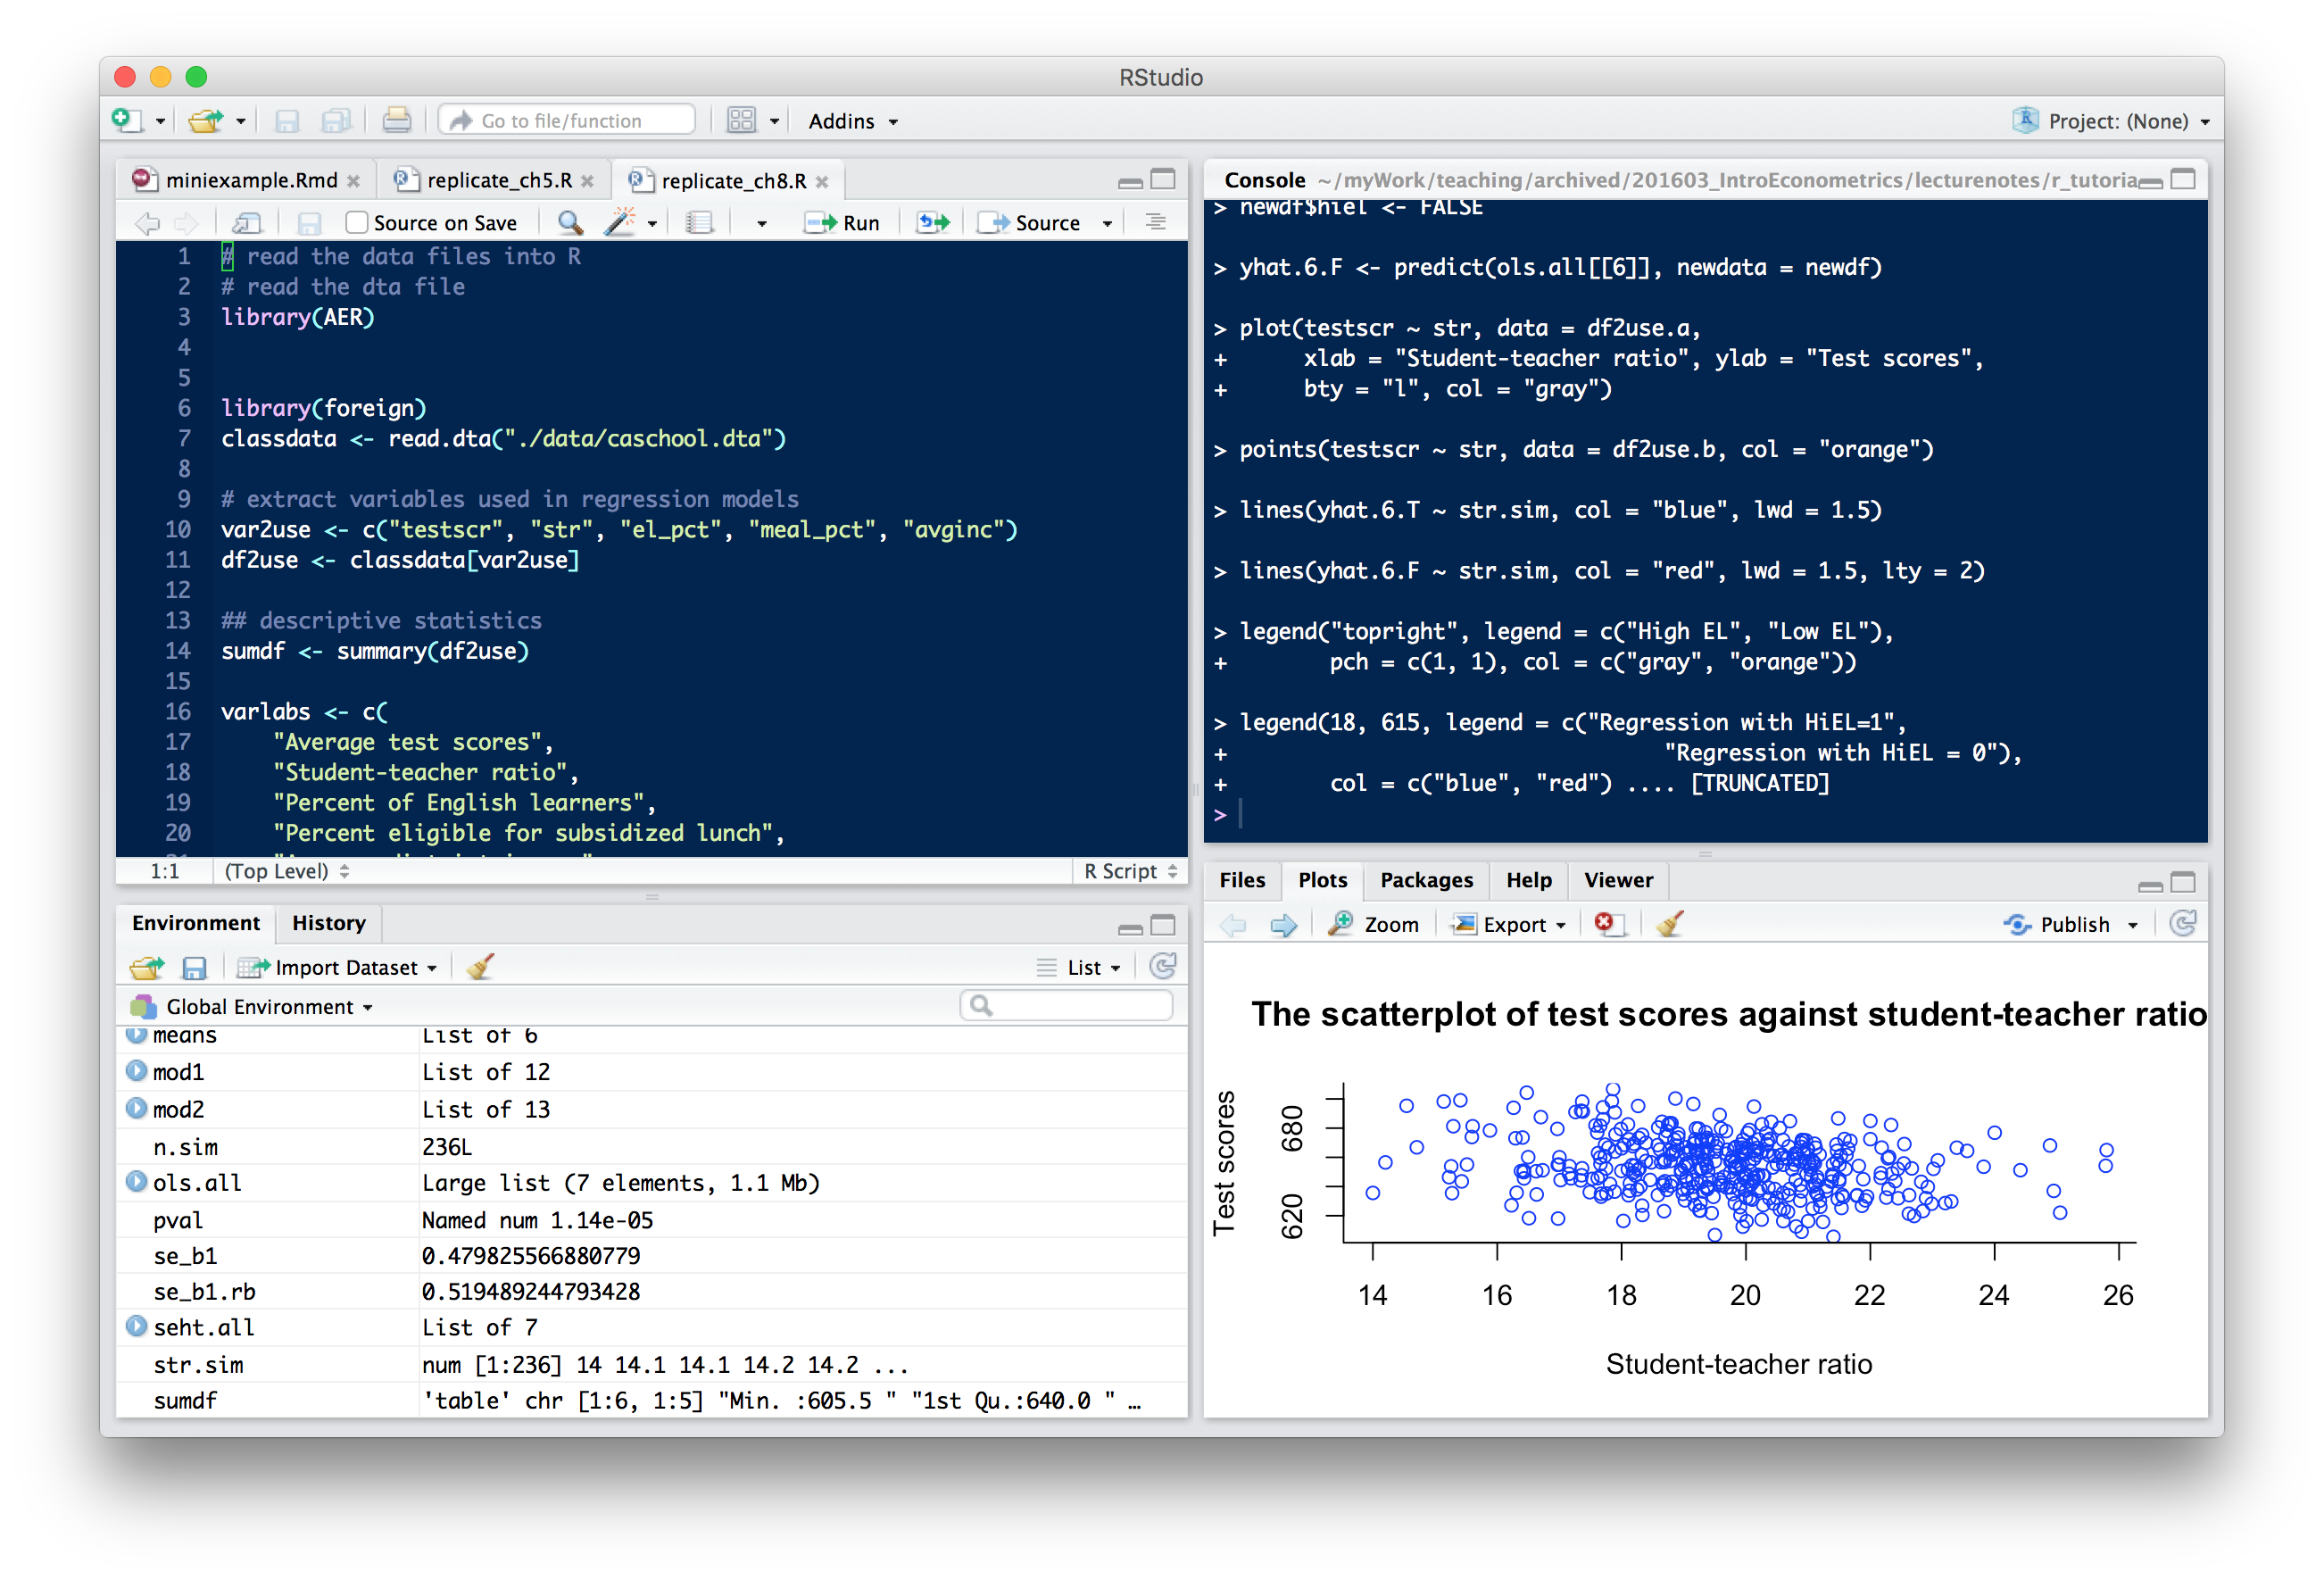
\includegraphics[width=0.95\textwidth]{figure/rstudio.png}
\caption{\label{fig:orgc66a6e6}
The Window of RStudio}
\end{figure}
\end{itemize}


\subsection{Packages}
\label{sec:org2c769af}

The R installation files install the core packages that support very
basic functions. One of the strength of R is that there are many
contributed packages written by the huge community of R users.

To install a contributed package, we use the command
\texttt{install.packages("names of packages")}. After installing a package,
we need to invoke it every time we use it by the command \texttt{library(name
of a package)}. In this course, for example, we need to install a
package called \texttt{AER} (Applied Econometrics with R).

Type the following code in the "Console" window in RStudio.

\begin{verbatim}
# Install packages
install.packages("AER")
\end{verbatim}

Upon typing this command, a window jumps up for you to choose a
mirror. From the list, choose China[Beijing]. R will automatically
download and install this package from the server. Very likely, when
this is the first package you install in R, R will also download other
packages on which installing the \texttt{AER} package depends. In the
console, you should see the following messages.

\begin{verbatim}
trying URL 'https://mirrors.tuna.tsinghua.edu.cn/CRAN/bin/macosx/mavericks/contrib/3.3/AER_1.2-5.tgz'
Content type 'application/octet-stream' length 2442603 bytes (2.3 MB)
==================================================
downloaded 2.3 MB


The downloaded binary packages are in
	/var/folders/rd/53x_sgqd3yj6wghsyyy4n0vh0000gn/T//RtmpF3tVDW/downloaded_packages
\end{verbatim}

In RStudio, you can install packages from the "Tools" menu and click
"Install Packages".

When we need to use the \texttt{AER} package, type \texttt{library(AER)} in the
console. And we can check whether this package is loaded using
\texttt{search()}.

\begin{verbatim}
# Load packages
library(AER)

# Check packages loaded
search()
\end{verbatim}

\begin{verbatim}
 [1] ".GlobalEnv"        "package:AER"       "package:survival"
 [4] "package:sandwich"  "package:lmtest"    "package:zoo"
 [7] "package:car"       "package:foreign"   "ESSR"
[10] "package:stats"     "package:graphics"  "package:grDevices"
[13] "package:utils"     "package:datasets"  "package:methods"
[16] "Autoloads"         "package:base"
\end{verbatim}

It shows that besides the \texttt{AER} package, there are other packages
in the "global" environment, which are the core packages loaded
automatically when opening R.


\subsection{Help}
\label{sec:org58bb39c}

\begin{itemize}
\item R has easy helping facilities. The help information of any function
can be found by type either \texttt{help()} or \texttt{?}.
\item If you cannot remember the accurate name of a function, you can even
guess by using \texttt{help.search()} or \texttt{??} or \texttt{apropos()}.
\item Any time you encounter a problem using R which cannot be solved by
\texttt{help} command, there are at least two places you can resort to.
\begin{itemize}
\item The mailing list of R: \url{http://www.r-project.org/mail.html}
\item Google or bing: quite often you will get an answer to your
question in the website of \url{http://stackoverflow.com/}.
\end{itemize}
\end{itemize}


\section{Basics}
\label{sec:org803fac9}

\subsection{R as a calculator}
\label{sec:org8da9543}

\subsubsection*{Standard arithmetic operators}
\label{sec:org0402dbf}

R supports the following arithmetic operators
\begin{verbatim}
+, -, *, /, ^, %%, %/%
\end{verbatim}

Hence,
\begin{verbatim}
## R as a calculator ------------------------------

#+ Binary operations
1 + 2; 2*3; 2^3; 5/2;
5 %% 2  # get x mod y
5 %/% 2 # get the integer division
\end{verbatim}

\begin{verbatim}
[1] 3
[1] 6
[1] 8
[1] 2.5
[1] 1
[1] 2
\end{verbatim}

\subsubsection*{Mathematical functions}
\label{sec:org8ad50c9}

R also have many built-in mathematical functions, such as, \texttt{log()},
\texttt{exp()}, \texttt{sin()}, \texttt{sqrt()}, \texttt{min()}, etc.

\begin{verbatim}
# Use built-in functions
log(exp(sin(pi/2)^2) * exp(cos(pi/3)^2))
\end{verbatim}

\begin{verbatim}
[1] 1.25
\end{verbatim}


\subsection{Vector operations}
\label{sec:org5f62bda}

Vector is the basic unit in R, from which other data structures,
for example, \texttt{matrix}, \texttt{factor}, \texttt{list}, \texttt{data.frame}, are built upon.

\subsubsection*{Generate a vector}
\label{sec:org46087c5}

A vector can be generated by the function \texttt{c()}, which can also be
used to concatenate two vectors

\begin{verbatim}
## Vector operations ------------------------------

# Create a vector with c()
x <- c(0.3, 1.5, 7.3, 2)
y <- c(3, 2, 1)
z <- c(x, y)
z
\end{verbatim}

\begin{verbatim}
[1] 0.3 1.5 7.3 2.0 3.0 2.0 1.0
\end{verbatim}

The symbol \texttt{<-} is to assign a value to a variable. You can also use
\texttt{=} to assign values, but \texttt{<-} is more commonly used by convention and
\texttt{=} is used within a function calling for assigning values to the
arguments of the function.

Note that by concatenating \texttt{x} and \texttt{y}, integers are converted to
floating point numbers. That means the elements in a vector must have
the same mode (data types), including \texttt{numeric}, \texttt{character}, and
\texttt{logical}.

\begin{verbatim}
# Vectors with different data types
student.names <- c("John", "Mary", "Bob", "Ann")
student.male <- c(TRUE, FALSE, TRUE, FALSE)
student.age <- c(20, 19, 21, 20)

class(student.names)
class(student.male)
class(student.age)

students <- c(student.names, student.male, student.age)
students
\end{verbatim}

\begin{verbatim}
[1] "character"
[1] "logical"
[1] "numeric"
 [1] "John"  "Mary"  "Bob"   "Ann"   "TRUE"  "FALSE" "TRUE"  "FALSE" "20"
[10] "19"    "21"    "20"
\end{verbatim}

\subsubsection*{Patterned vectors}
\label{sec:org18517cc}

A vector can also be generated by the functions, like \texttt{rep()}, \texttt{seq()}, and
\texttt{:}.

\begin{itemize}
\item \texttt{seq()} generates a vector by some patterns and \texttt{a:b} is a shorthand
for \texttt{seq(from=a, to=b, by=1)}.

\begin{verbatim}
# Create a sequence
even <- seq(from = 2, to = 20, by = 2)
even
years <- 1995:2005
years
\end{verbatim}

\begin{verbatim}
[1]  2  4  6  8 10 12 14 16 18 20
[1] 1995 1996 1997 1998 1999 2000 2001 2002 2003 2004 2005
\end{verbatim}

\item \texttt{rep()} generates a vector by repeating some values

\begin{verbatim}
# Create repetition
ones <- rep(1, times = 10)
ones
rep13 <- rep(1:3, times = 3, each = 2)
rep13
\end{verbatim}

\begin{verbatim}
[1] 1 1 1 1 1 1 1 1 1 1
[1] 1 1 2 2 3 3 1 1 2 2 3 3 1 1 2 2 3 3
\end{verbatim}
\end{itemize}

\subsubsection*{Vector operations}
\label{sec:orgee63d64}

Arithmetic operators and mathematical functions can be applied to
vector in an element-by-element way in R.

Let's first draw random numbers for the uniform distribution
\(x \sim Uniform(0, 1)\). The length of \(x\) is 10. We can use the
\texttt{length()} function to check the length of a vector.

\begin{verbatim}
# Draw a random vector
x <- runif(10); x
length(x)
\end{verbatim}

\begin{verbatim}
 [1] 0.7509281 0.5274957 0.2658100 0.8538053 0.1332318 0.6500801 0.3687549
 [8] 0.4117108 0.2145863 0.1970263
[1] 10
\end{verbatim}

The arithmetic operations and built-in math functions are all applied
for each element of a vector.
\begin{verbatim}
2 * x + 3
log(x)
\end{verbatim}

\begin{verbatim}
[1] 4.501856 4.054991 3.531620 4.707611 3.266464 4.300160 3.737510 3.823422
[9] 3.429173 3.394053
[1] -0.2864454 -0.6396146 -1.3249734 -0.1580521 -2.0156646 -0.4306598
[7] -0.9976230 -0.8874342 -1.5390434 -1.6244179
\end{verbatim}

If two vectors with different lengths are computed within one
operation, the elements of the vector with a shorter length will be
used in an iterated way. We must keep in mind this feature of R, which
in some cases may give rise to unintended results.

\begin{verbatim}
y <- runif(5)
x + y
\end{verbatim}

\begin{verbatim}
[1] 0.8556952 1.2264015 0.9013787 1.3446773 0.4927895 0.7548471 1.0676607
[8] 1.0472795 0.7054582 0.5565840
\end{verbatim}

\subsubsection*{Selecting elements in a vector}
\label{sec:org1911752}

Element(s) in a vector can be selected by \texttt{[position]}, in which
\texttt{position} can be a vector indicating the position of each element in
a vector, a negative value to exclude an element with the
corresponding position, and a condition to select elements satisfying
the condition.

\begin{verbatim}
# Selecting elements in a vector
x[1:5]
x[c(1, length(x))]
x[-4]
x[x > 0.5]
\end{verbatim}

\begin{verbatim}
[1] 0.7509281 0.5274957 0.2658100 0.8538053 0.1332318
[1] 0.7509281 0.1970263
[1] 0.7509281 0.5274957 0.2658100 0.1332318 0.6500801 0.3687549 0.4117108
[8] 0.2145863 0.1970263
[1] 0.7509281 0.5274957 0.8538053 0.6500801
\end{verbatim}

Instead of selecting elements in a vector by their positions, we can
also give each element a particular name so that we can use their
names to choose elements.

\begin{verbatim}
student.names
student.age
# Give elements names
names(student.age) <- student.names
student.age
student.age[c("John", "Bob")]
\end{verbatim}

\begin{verbatim}
[1] "John" "Mary" "Bob"  "Ann"
[1] 20 19 21 20
John Mary  Bob  Ann
  20   19   21   20
John  Bob
  20   21
\end{verbatim}


\subsection{Matrices}
\label{sec:org389889b}

\subsubsection*{Create a matrix}
\label{sec:org333a288}

We can create a matrix with the \texttt{matrix()} function, in which the
first argument is a vector. We specify the
two dimensions by the arguments of \texttt{nrow} and \texttt{ncol}. By default,
\texttt{matrix()} arranges all the elements of the vector in its first
argument into a matrix by column. We can change it by adding
\texttt{byrow=TRUE}.

\begin{verbatim}
# Create a matrix
A <- matrix(1:12, nrow = 3, ncol = 4); A
matrix(1:12, nrow = 3, ncol = 4, byrow = TRUE)
\end{verbatim}

\begin{verbatim}
     [,1] [,2] [,3] [,4]
[1,]    1    4    7   10
[2,]    2    5    8   11
[3,]    3    6    9   12
     [,1] [,2] [,3] [,4]
[1,]    1    2    3    4
[2,]    5    6    7    8
[3,]    9   10   11   12
\end{verbatim}

We can also juxtapose vectors of the same length to create a matrix by
\texttt{cbind()}, or stack over vectors by \texttt{rbind()}.

\begin{verbatim}
# Create a matrix by combining vectors
a <- 1:4; b <- 2:5; c <- 3:6
cbind(a, b, c)
rbind(a, b, c)
\end{verbatim}

\begin{verbatim}
     a b c
[1,] 1 2 3
[2,] 2 3 4
[3,] 3 4 5
[4,] 4 5 6
  [,1] [,2] [,3] [,4]
a    1    2    3    4
b    2    3    4    5
c    3    4    5    6
\end{verbatim}

Like vectors, we can also give each row and each column in a matrix
their specific names. Here we use the function of \texttt{paste()} to combine
two (character) vectors together to generate a new character vector.

\begin{verbatim}
# Give names to rows and columns
rownames(A) <- paste("X", 1:3, sep = "")
colnames(A) <- paste("Y", 1:4, sep = "")
A
\end{verbatim}

\begin{verbatim}
   Y1 Y2 Y3 Y4
X1  1  4  7 10
X2  2  5  8 11
X3  3  6  9 12
\end{verbatim}

\subsubsection*{Select elements}
\label{sec:orgc0425b1}

We select elements from a matrix using \texttt{[rows, cols]}. \texttt{rows} and
\texttt{cols} are two vectors to set the rows and columns of elements to be
selected.

\begin{verbatim}
# Selecting elements in a matrix
A[1, 3]
A["X1", "Y3"]
A[1:3, c(2, 4)]
A[, 2]
A[3, ]
\end{verbatim}

\begin{verbatim}
[1] 7
[1] 7
   Y2 Y4
X1  4 10
X2  5 11
X3  6 12
X1 X2 X3
 4  5  6
Y1 Y2 Y3 Y4
 3  6  9 12
\end{verbatim}

\subsubsection*{Matrix operations}
\label{sec:org0f3a9d3}

We can do all matrix operations that we have reviewed in Lecture 4.

\begin{itemize}
\item Transpose
\label{sec:org6714e0b}

\begin{verbatim}
t(A)
\end{verbatim}

\begin{verbatim}
   X1 X2 X3
Y1  1  2  3
Y2  4  5  6
Y3  7  8  9
Y4 10 11 12
\end{verbatim}

\item Matrix multiplication
\label{sec:org1e3d403}

There are two types of matrix multiplication. The \texttt{*} operator
computes the element-by-element multiplication (Hadamard product),
while the operator \texttt{\%*\%} computes matrix multiplication in the form of
inner products of row and column vectors.

When we do either type of matrix multiplication, we should always
check whether the two matrices are conformable to do so. If not, R
will give you an error message. We can use the function \texttt{dim()} to see
the dimensions of a matrix.

\begin{verbatim}
B <- matrix(1:8, nrow = 4)
A * B # element-by-element multiplication
dim(A)
dim(B)
\end{verbatim}

\begin{verbatim}
Error in A * B : non-conformable arrays
[1] 3 4
[1] 4 2
\end{verbatim}

\begin{verbatim}
A %*% B
\end{verbatim}

\begin{verbatim}
   [,1] [,2]
X1   70  158
X2   80  184
X3   90  210
\end{verbatim}

\item Inverse matrix
\label{sec:orgde5d808}

We use the function \texttt{solve(A)} to get the inverse matrix of
\(\mathbf{A}\).

\begin{verbatim}
A <- matrix(rnorm(9), nrow = 3)
B <- solve(A)
A %*% B
\end{verbatim}

\begin{verbatim}
             [,1]         [,2]          [,3]
[1,] 1.000000e+00 0.000000e+00  0.000000e+00
[2,] 0.000000e+00 1.000000e+00 -2.220446e-16
[3,] 3.330669e-16 2.775558e-17  1.000000e+00
\end{verbatim}

Notice that the resultant matrix is not exactly an identity matrix, in
which some off-diagonal elements are very small non-zero
numbers. These are the rounding errors stemming from conversion
between binary bits (a sequence of 0 and 1) to floating point
numbers.

\texttt{solve()} can also be used to solve a system of linear equations, such
as,
\begin{align*}
3x &+ 2y - z   = 1 \\
2x &- 2y + 4z  = -2 \\
-x &+ \frac{1}{2}y - z  = 0
\end{align*}
to which the solution is \(x=1, y=-2, z=-2\).

The system of equations can be written in matrix notation as
\begin{equation*}
\begin{bmatrix}
3 & 2 & -1 \\
2 & -2 & 4 \\
-1 & \frac{1}{2} & -1
\end{bmatrix}
\begin{bmatrix}
x \\
y \\
z
\end{bmatrix}
=
\begin{bmatrix}
1 \\
-2 \\
0
\end{bmatrix}
\end{equation*}

\begin{verbatim}
A <- cbind(c(3, 2, -1),
	   c(2, -2, 0.5),
	   c(-1, 4, -1))
B <- c(1, -2, 0)
solve(A, B)
\end{verbatim}

\begin{verbatim}
[1]  1 -2 -2
\end{verbatim}
\end{itemize}

\subsubsection*{Diagonal matrix}
\label{sec:org4c85be1}

The function \texttt{diag()} can create a diagonal matrix.

\begin{verbatim}
diag(1:3)
\end{verbatim}

\begin{verbatim}
     [,1] [,2] [,3]
[1,]    1    0    0
[2,]    0    2    0
[3,]    0    0    3
\end{verbatim}

An identity matrix is a special case of a diagonal matrix.

\begin{verbatim}
diag(3)
\end{verbatim}

\begin{verbatim}
     [,1] [,2] [,3]
[1,]    1    0    0
[2,]    0    1    0
[3,]    0    0    1
\end{verbatim}

\subsubsection*{Higher-dimensional array}
\label{sec:org51cf395}

Vectors and matrices are special cases of arrays. The former is
one-dimensional array, and the latter is two-dimensional. We can also
create higher-dimensional arrays by \texttt{array()}.

\begin{verbatim}
array(1:18, dim = c(3, 3, 2))
\end{verbatim}

\begin{verbatim}
, , 1

     [,1] [,2] [,3]
[1,]    1    4    7
[2,]    2    5    8
[3,]    3    6    9

, , 2

     [,1] [,2] [,3]
[1,]   10   13   16
[2,]   11   14   17
[3,]   12   15   18
\end{verbatim}


\subsection{List}
\label{sec:org0ee932c}

Vectors, matrices, and arrays are all the ways of R to store
data. However, their limitation is obvious, all elements in a vector
or a matrix must be of the same type. To overcome this limitation, R
uses another way to store data, called a \texttt{list}.

Here is how we create a list, which consists of three components, a
character vector \texttt{chr}, a numeric vector \texttt{num}, and a logical vector
\texttt{boo}. Note that the lengths of all components do not need to be
equal.

\begin{verbatim}
mylist <- list(chr = c("a", "b", "c", "d"),
	       num = 1:10,
	       boo = c(TRUE, FALSE, FALSE, TRUE))
mylist
\end{verbatim}

\begin{verbatim}
$chr
[1] "a" "b" "c" "d"

$num
 [1]  1  2  3  4  5  6  7  8  9 10

$boo
[1]  TRUE FALSE FALSE  TRUE
\end{verbatim}

To select a component, we use the \texttt{\$=operator or =[[]]}.

\begin{verbatim}
mylist$chr
mylist[[2]][3:6]
mylist[["boo"]][-1]
\end{verbatim}

\begin{verbatim}
[1] "a" "b" "c" "d"
[1] 3 4 5 6
[1] FALSE FALSE  TRUE
\end{verbatim}


\section{Data Management in R}
\label{sec:org4649e4d}

R use data frames as its main device to save a whole data set,
especially data read from an external file. A data frame is a mixture
of a list and a matrix. As a list, a data frame can include different
types of data and use the \texttt{\$} or \texttt{[[]]} operator to select a component
that is a variable in the data set. As a matrix, all variables in a
data frame should have the same length and are arranged in a matrix
format.

\subsection{Create a data frame}
\label{sec:org9a66545}

We can manually create a data frame object, convert a matrix to a data
frame object, or read data in an external file into R and save them in
a data frame object.

\subsubsection*{Create a data frame manually}
\label{sec:org2d3e169}
\begin{verbatim}
mydata <- data.frame(X = 1:5, Y = letters[1:5], Z = rep(c(TRUE, FALSE), length = 5)); mydata
\end{verbatim}

\begin{verbatim}
  X Y     Z
1 1 a  TRUE
2 2 b FALSE
3 3 c  TRUE
4 4 d FALSE
5 5 e  TRUE
\end{verbatim}

\subsubsection*{Convert a matrix to a data frame}
\label{sec:orgbca290f}

We use \texttt{as.data.frame()} to convert a matrix to a data frame. In
creating the matrix, we use \texttt{sample.int()} that is a special case of
the function \texttt{sample()} to draw random samples from a vector.
\begin{verbatim}
A <- matrix(sample.int(100, size = 20), nrow = 5)
A.df <- as.data.frame(A); A.df
\end{verbatim}

\begin{verbatim}
  V1 V2 V3 V4
1 39 69 96 16
2 91 77 98 26
3 73 36 40 95
4 24 21 15  4
5 65 33 37  8
\end{verbatim}

We can assign each variable (column) a name. Here we use the function
\texttt{paste()} to combine a string \texttt{VAR} with each element of the vector
\texttt{1:4}, joined with \texttt{\_}.
\begin{verbatim}
names(A.df) <- paste("VAR", 1:4, sep = "_"); A.df
\end{verbatim}

\begin{verbatim}
  VAR_1 VAR_2 VAR_3 VAR_4
1    39    69    96    16
2    91    77    98    26
3    73    36    40    95
4    24    21    15     4
5    65    33    37     8
\end{verbatim}


\subsection{Read data from a file}
\label{sec:org19bd2eb}

Suppose we have a data file, \url{mydata.txt}. We can read the data
directly from the file using the function \texttt{read.table()}. Upon reading
the data into R, we should check whether data are correctly using the
function \texttt{head()} to check the first few (default is six)
observations. (or )

\begin{verbatim}
mydata <- read.table("mydata.txt", header = TRUE, sep = "")
head(mydata)
# tail(mydata)
\end{verbatim}

\begin{verbatim}
  Names Gender Weight Overweight
1   Bob      M   72.5      FALSE
2  John      M   83.1      FALSE
3  Anne      F   60.8      FALSE
4   Dan      M   89.7       TRUE
5  Juan      M   93.2       TRUE
6  Jane      F   76.9       TRUE
\end{verbatim}

Often we may encounter data files ending with \texttt{.csv}, which is a
special type of a text file, with commas separating each value. And we
use the function \texttt{read.csv()} to read a \texttt{.csv} file.

\begin{verbatim}
tail(read.csv("mydata.csv", header = TRUE))
\end{verbatim}

\begin{verbatim}
  Names Gender Weight Overweight
2  John      M   83.1      FALSE
3  Anne      F   60.8      FALSE
4   Dan      M   89.7       TRUE
5  Juan      M   93.2       TRUE
6  Jane      F   76.9       TRUE
7 Doris      F   56.3      FALSE
\end{verbatim}

We can also read data from an excel file or a Stata file that we will
see in the final section of this tutorial. To read these types of
files, we need to load the packages of \texttt{gdata}, \texttt{foreign} (for Stata
12 and prior version), or \texttt{readstata13} (for Stata 13 and newer
version).
\begin{verbatim}
library(gdata)
read.xls(mydata.xls)

library(foreign)
read.dta(mydata.dta)
\end{verbatim}


\subsection{Select variables}
\label{sec:org5cccfbc}

Since a data frame is a special case of list, we can select a variable
in a data frame by using "\texttt{\$}" or "\texttt{[[]]}". Here is an example of
computing the average weight of students.

\begin{verbatim}
mean(mydata$Weight)
\end{verbatim}

\begin{verbatim}
[1] 76.07143
\end{verbatim}


\subsection{Get summary information}
\label{sec:orgeb7951d}

After reading data into R, besides using \texttt{head()} or \texttt{tail()} to see
the first and last few observations, we need also use \texttt{str()} and
\texttt{summary()} to get some summary information of the data set.

\begin{verbatim}
str(mydata)
summary(mydata)
\end{verbatim}

\begin{verbatim}
'data.frame':	7 obs. of  4 variables:
 $ Names     : Factor w/ 7 levels "Anne","Bob","Dan",..: 2 6 1 3 7 5 4
 $ Gender    : Factor w/ 2 levels "F","M": 2 2 1 2 2 1 1
 $ Weight    : num  72.5 83.1 60.8 89.7 93.2 76.9 56.3
 $ Overweight: logi  FALSE FALSE FALSE TRUE TRUE TRUE ...
   Names   Gender     Weight      Overweight
 Anne :1   F:3    Min.   :56.30   Mode :logical
 Bob  :1   M:4    1st Qu.:66.65   FALSE:4
 Dan  :1          Median :76.90   TRUE :3
 Doris:1          Mean   :76.07   NA's :0
 Jane :1          3rd Qu.:86.40
 John :1          Max.   :93.20
 Juan :1
\end{verbatim}

The results of running \texttt{str()} show that the variables \texttt{Names} and
\texttt{Gender} have the type of \texttt{Factor}. In default, when reading
character variables from a file, R will convert them into factors that
are categorical variables. We can preserve the type of character by
including \texttt{stringsAsFactors=FALSE} in \texttt{read.table()} or \texttt{read.csv()}.


\section{Graphics}
\label{sec:org49a1899}

R is very powerful in creating graphics. In this tutorial, we will learn
base graphics systems in R.

We use a database, \texttt{mtcars}, in the \texttt{datasets} package in R to show
how to draw different types of graphics. This data set contain the
data that was extracted from the 1974 Motor Trend US magazine, and
comprises fuel consumption and 10 aspects of automobile design and
performance for 32 automobiles (1973–74
models).(Read \url{https://stat.ethz.ch/R-manual/R-devel/library/datasets/html/mtcars.html})

\begin{verbatim}
data(mtcars)
head(mtcars)
# str(mtcars)
\end{verbatim}

\begin{verbatim}
                   mpg cyl disp  hp drat    wt  qsec vs am gear carb
Mazda RX4         21.0   6  160 110 3.90 2.620 16.46  0  1    4    4
Mazda RX4 Wag     21.0   6  160 110 3.90 2.875 17.02  0  1    4    4
Datsun 710        22.8   4  108  93 3.85 2.320 18.61  1  1    4    1
Hornet 4 Drive    21.4   6  258 110 3.08 3.215 19.44  1  0    3    1
Hornet Sportabout 18.7   8  360 175 3.15 3.440 17.02  0  0    3    2
Valiant           18.1   6  225 105 2.76 3.460 20.22  1  0    3    1
\end{verbatim}


\subsection{The barchart}
\label{sec:org87373d5}

First, Let's see the mpg (miles per gallon) among different models by
the bar chart.

\begin{verbatim}
barplot(sort(mtcars$mpg, decreasing = TRUE),
	col = "blue",
	main = "The mpg among car models",
	xlab = "car models", ylab = "mpg")
\end{verbatim}

\begin{center}
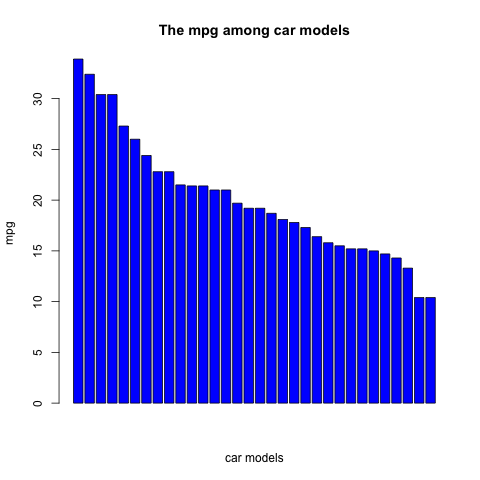
\includegraphics[width=0.8\textwidth]{figure/barplot.png}
\end{center}


\subsection{The scatterplot}
\label{sec:org2e513fa}

We know in Lecture 3 that a scatterplot is often used to see the
association between two variables. Let's see the relationship between
miles per gallon, \texttt{mpg}, and car weights, \texttt{disp}.

\begin{verbatim}
plot(mtcars$wt, mtcars$mpg,
     main = "The scatterplot between mpg and displacement",
     xlab = "Car weights (lbs/1000)",
     ylab = "Miles per gallon",
     pch = 19, col = "red")
\end{verbatim}

\begin{center}
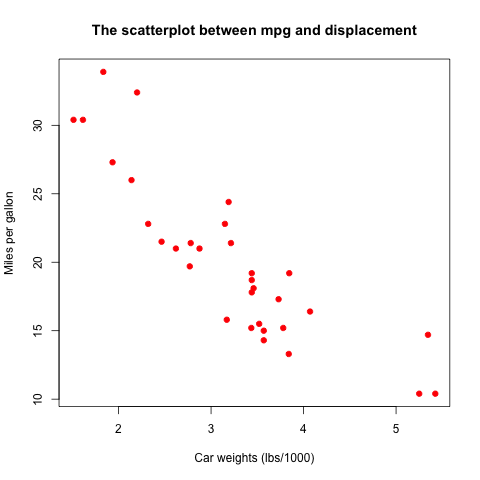
\includegraphics[width=0.8\textwidth]{figure/scatterplot.png}
\end{center}

We will explore more graphic capabilities of R in the lectures to
come.



\section{Statistical Analysis}
\label{sec:org11c63a1}

Now we can show how to use R to do some statistical
analysis. This demonstration answers the questions of Empirical
Exercise 3.1 at the end
of Chapter 3. Furthermore, we carry out this exercise in the format of
\textbf{reproducible research}. That means, we should accomplish they
following tasks in answering the problem:
\begin{enumerate}
\item using R to compute the statistics
asked in the questions
\item including R code and the results of running the code in the answer, and
\item describing our work and answers in plain language along with code
and numerical answers.
\end{enumerate}


\subsection{A description of the problem}
\label{sec:orgc3372da}

Empirical exercise 3.1 concerns the relationship between average
earnings and education levels, using the data set from the 1992 and
2008 Current Population Survey (CPS). Specifically, we want to see
whether the average hourly earnings (\texttt{ahe}) are different between
workers with a bachelor degree and those with only high school
diploma (\texttt{bachelor}).

\subsection{Answers to the questions}
\label{sec:org2ee93e6}

\subsubsection*{Question (a)}
\label{sec:org5bb9dc0}

\begin{verse}
Compute the sample mean for average hourly earnings (\texttt{ahe}) in 1992 and\\
in 2008. Construct a 95\% confidence interval for the population means\\
for \texttt{ahe} in 1992 and 2008 and the change between 1992 and 2008\\
\end{verse}

\begin{itemize}
\item Read the data
\label{sec:orgb4bc8f0}

The first thing first is of course read the data correctly from the
Stata file \url{data/cps92\_08.dta}, which can be read by the function
\texttt{read.dta()} in the package of \texttt{foreign}.

\begin{verbatim}
library(foreign)
cpsdat <- read.dta("data/cps92_08.dta")
head(cpsdat)
\end{verbatim}

\begin{verbatim}
  year       ahe bachelor female age
1 1992 11.188811        1      0  29
2 1992 10.000000        1      0  33
3 1992  5.769231        0      0  30
4 1992  1.562500        0      0  32
5 1992 14.957265        1      0  31
6 1992  8.660096        1      1  26
\end{verbatim}

\item Calculate the sample means of average hourly earnings in 1992 and 2008
\label{sec:orgbc0eb9d}

There are many ways to compute the sample means in 1992 and 2008,
respectively. First, to make you more familiar with the  R
language, we compute them in a very basic way. Then, we show how to
get the same results with some powerful functions.

\begin{verbatim}
# extract the data for average hourly earnings in 1992 and 2008
ahe.92 <- cpsdat$ahe[cpsdat$year == 1992]
ahe.08 <- cpsdat$ahe[cpsdat$year == 2008]
mean.ahe.92 <- mean(ahe.92); mean.ahe.92
mean.ahe.08 <- mean(ahe.08); mean.ahe.08
\end{verbatim}

\begin{verbatim}
[1] 11.62637
[1] 18.97609
\end{verbatim}

The average hourly earnings are \texttt{11.63} dollars
in 1992 and \texttt{18.98} dollars in 2008.

\item Construct the confidence intervals
\label{sec:orgeecdc6b}

Recall that a 95\% confidence interval for the population mean can be
constructed as \(\overline{Y} \pm 1.96 SE(\overline{Y})\) and
\(SE(\overline{Y})\) is computed as \(s_Y / \sqrt{n}\).

\begin{verbatim}
# the sample variance
sd.ahe.92 <- sd(ahe.92)
sd.ahe.08 <- sd(ahe.08)

n.92 <- length(ahe.92)
n.08 <- length(ahe.08)

# the standard error
se.ahe.92 <- sd.ahe.92 / sqrt(n.92)
se.ahe.08 <- sd.ahe.08 / sqrt(n.08)

# 95% confidence interval
# the 95% critical value from a normal distribution
cv.95 <- qnorm(0.975)

lower.lim.92 <- mean.ahe.92 - cv.95 * se.ahe.92
lower.lim.08 <- mean.ahe.08 - cv.95 * se.ahe.08

upper.lim.92 <- mean.ahe.92 + cv.95 * se.ahe.92
upper.lim.08 <- mean.ahe.08 + cv.95 * se.ahe.08
\end{verbatim}

The 95\% confidence interval for \texttt{ahe} in 1992 is
(\texttt{11.5}, \texttt{11.75}), and
that in 2008 is (\texttt{18.75},
\texttt{19.2}).

\item Alternative methods to calculate the sample means and confidence intervals
\label{sec:orgacb4dd7}

In the above example, to compute the sample averages in 1992 and 2008,
we write code separately for each year, which can be done more easily
in R.

We can compute the averages for each year using the function
\texttt{aggregate()}, which splits the whole data base into two parts by the
values of \texttt{year}. Then, for each part we compute the average by
specifying the argument \texttt{FUN} to be \texttt{mean}, i.e., specifying the
function to be used for each part as the \texttt{mean()} function. Also, in
this case, we use \texttt{\textasciitilde{}} to specify a \textbf{formula} that means that we split
\texttt{ahe} by \texttt{year}.

\begin{verbatim}
# Use aggregate() to compute the means in both years
ahe.means <- aggregate(ahe ~ year, FUN = mean, data = cpsdat)
ahe.means
\end{verbatim}

\begin{verbatim}
  year      ahe
1 1992 11.62637
2 2008 18.97609
\end{verbatim}

The confidence interval can be extracted from the results of the
\texttt{t.test()} function, which is a list.
\begin{verbatim}
# t test for ahe in 1992
t.ahe.92 <- t.test(ahe.92); t.ahe.92$conf.int
# t test for ahe in 2008
t.ahe.08 <- t.test(ahe.08); t.ahe.08$conf.int
# test for the change between 1992 and 2008
t.ahe.diff <- t.test(ahe.08, ahe.92); t.ahe.diff
\end{verbatim}

\begin{verbatim}
[1] 11.50019 11.75254
attr(,"conf.level")
[1] 0.95
[1] 18.74975 19.20244
attr(,"conf.level")
[1] 0.95

	Welch Two Sample t-test

data:  ahe.08 and ahe.92
t = 55.597, df = 12065, p-value < 2.2e-16
alternative hypothesis: true difference in means is not equal to 0
95 percent confidence interval:
 7.090601 7.608853
sample estimates:
mean of x mean of y
 18.97609  11.62637
\end{verbatim}

The confidence interval of the change in average hourly earnings
between 1992 and 2008 is (\texttt{7.09},
\texttt{7.61}).
\end{itemize}

\subsubsection*{Question (b)}
\label{sec:org8f6512b}

Now we need to adjust the average hourly earnings in the 1992 dollars
to the 2008 dollars with the inflation rate, computed as
\texttt{CPI2008/CPI1992}.

\begin{verbatim}
# CPI in 1992 and 2008
cpi.92 <- 140.3
cpi.08 <- 215.2
# Inflation adjustment
inflator <- cpi.08 / cpi.92
cpsdat$ahe.adj <- with(cpsdat, ifelse(year == 1992, ahe * inflator, ahe))
\end{verbatim}

In the code block above, we first use the function \texttt{with()} to attach
the data frame \texttt{cpsdat} within its own environment so that when we
refer to variables in \texttt{cpsdat}, such as \texttt{ahe} and \texttt{year}, we do not
need to write \texttt{cpsdat\$} and every time we use its variables.

The function \texttt{ifesle()} set the values of \texttt{ahe} based on the
condition \texttt{year == 1992}. If the condition is true, we do \texttt{ahe *
inflator}; if not, leave \texttt{ahe} as it is.

Then we repeat what we've done in Question (a) with the
inflation-adjusted earnings in 1992.

\begin{verbatim}
ahe.92.adj <- with(cpsdat, ahe.adj[year == 1992])
mean.ahe.92.adj <- mean(ahe.92.adj)
t.ahe.92.adj <- t.test(ahe.92.adj)
t.ahe.diff.adj <- t.test(ahe.08, ahe.92.adj)
\end{verbatim}

\begin{itemize}
\item The sample average of the inflation-adjusted earnings in 1992 is
\texttt{17.83} in the 2008 dollars.

\item The confidence interval for the inflation-adjusted average hourly earnings in 1992 is
(\texttt{17.64, 18.03}).

\item The confidence interval for the change between 1992 and 2008 is
(\texttt{0.85, 1.44}).
\end{itemize}

\subsubsection*{Question (c)}
\label{sec:org43f90bf}

If we are interested in the change in workers' purchasing power, the
results with the inflation-adjusted earnings should be used in
comparison.

\subsubsection*{Question (d)}
\label{sec:org2b78704}

Now let's compute the average earnings for high school graduates and
college graduates with the 2008 data. First thing to do is to select
the 2008 data from \texttt{cpsdat} using the function \texttt{subset()}

\begin{verbatim}
# select data in 2008
cps08 <- subset(cpsdat, year == 2008, select = c(year, ahe, bachelor))

# calculate means
ahe.educ.08 <- aggregate(ahe ~ bachelor, FUN = mean, data = cps08)

# select ahe and filter by bachelor
ahe.high.08 <- with(cps08, ahe[bachelor == 0])
ahe.bach.08 <- with(cps08, ahe[bachelor == 1])

# construct confindence interval
t.ahe.high.08 <- t.test(ahe.high.08)
t.ahe.bach.08 <- t.test(ahe.bach.08)
t.ahe.gap.08  <- t.test(ahe.bach.08, ahe.high.08)
\end{verbatim}

\begin{itemize}
\item The mean of the average hourly earnings of high school graduates in
2008 is
\texttt{15.33}
dollars with the 95\% confidence interval
(\texttt{15.09, 15.57})

\item The mean of the average hourly earnings of college graduates is
\texttt{22.91}
dollars with the 95\%
confidence interval
(\texttt{22.56, 23.26})

\item The 95\% confidence interval of the gap in earnings between the two
groups is
(\texttt{7.15, 8})
\end{itemize}

We can create a boxplot to compare the means and confidence intervals
of average hourly earnings between high school graduates and college
graduates.

\begin{verbatim}
boxplot(ahe ~ bachelor, data = cps08,
	main = "Average Hourly Earnings by Education",
	col = c("red", "orange"),
	xlab = "Bachelor degres = 1, high school = 0",
	ylab = "US$ 2008")
\end{verbatim}

\begin{center}
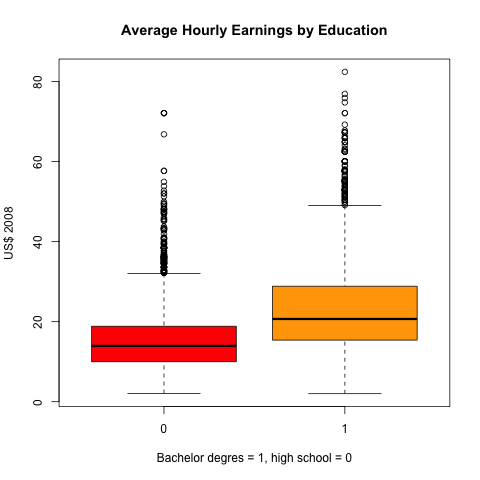
\includegraphics[width=.9\linewidth]{figure/boxplot.png}
\end{center}

We leave Question (e)-(g) to students as exercises.

I include a \texttt{Rmd} file that can generate an html or pdf file from
RStudio. \url{mdfiles/emp\_3\_1.Rmd}
\end{document}